% !Tex root = Vorlage.tex
An investment strategy based on a Minimum Variance Portfolio seeks to minimize the risk of an investment. There is thus no desired target-return or stock-forecast to be considered. The portfolio optimization process can be described as pure risk-minimization, where the goal is a determination of the weight-distribution yielding the lowest possible risk at any time. Graphically, one can think of a Minimum Variance Portfolio as the most left point of the mean-variance-frontier.In this report, the minimum variance portfolio will be theoretically introduced and implemented in the R programming language. 

\section{Theory}
As written in the paper by DeMiguel et al.\cite{DEM09}, the weights were chosen according to the portfolio that minimizes the variance of return, e.g. 

\begin{equation} \label{eq:1}
\min_{w_t} w_t^{\perp}\Sigma_{t}w_{t}
\end{equation}

under the restriction that 

\begin{equation} \label{eq:2}
1_{N}^{\perp}w_{t} \overset{!}{=} 1
\end{equation}

and

\begin{equation} \label{eq:3}
\Sigma_t w_t \overset{!}{=} 1,
\end{equation}

where $w_t \in \mathbb{R}^{N}$ is the weight-vector at time $t \in \lbrace 1, 2, \dots, T \rbrace$ with $T \in \mathbb{N}$ period under observation and $N \in \mathbb{N}$ number of assets considered. $\Sigma_t \in \mathbb{N \times N}$ names the covariance matrix of excess-returns $R_{\tau} \in \mathbb{R}^{N \times \tau}$ at time $t$ for a subset $\tau$ of the period of Observation $\tau \subseteq \lbrace 1, 2, \dots, T \rbrace$. In the equation above, 1 is thought of as the N-dimensional vector containing 1s. \\

We now want to investigate the restriction $\min_{w_t}$for one fixed time-period T, such that $\tau = T$. As a result, weights are not time-dependent anymore. Note that when constructing a Minimum Variance Portfolio, weights are in fact time-dependent. However, for the sake of legibility, we will for now treat the case where $w_t = w$.\\

Considering three risky assets and a weight vector $w \in \mathbb{R}^{3}$, such that 
\begin{equation}
  w = \begin{pmatrix}w_1\\w_2\\w_3\end{pmatrix},
\end{equation}
the minimal variance restraint can then be interpreted as follows\cite[p.~7]{ZIV13}:
\begin{equation} \label{eq:4}
  \begin{split}
    \min_{w_1, w_2, w_3} \sigma^2_{w_1, w_2, w_3} = & w^2_1 \sigma^2_1 + w^2_2 \sigma^2_2 + w^2_3 \sigma^2_3 + \\ & 2w_1w_2 \sigma_{12} + 2w_1w_3\sigma_{13} + 2w_2w_3\sigma_{23}
  \end{split}
\end{equation}
Here, the components' variance $\sigma^2_{i}$ and standard deviation $\sigma_{i,j}$ for $i,j \in \lbrace 1, 2, 3 \rbrace$ are used to describe the relationship. The Lagrange-function of this problem can be written as 
\begin{equation} \label{eq:5}
  \begin{split}
    L(w_1, w_2, w_3, \lambda) = & w^2_1 \sigma^2_1 + w^2_2 \sigma^2_2 + w^2_3 \sigma^2_3 + \\ & 2w_1w_2 \sigma_{12} + 2w_1w_3\sigma_{13} + 2w_2w_3\sigma_{23} \\
    + & \lambda(w_1 + w_2 + w_3 - 1)
  \end{split}
\end{equation}

Now, the component-wise deviates can be found and be set to equal zero, yielding the first order conditions.

\begin{equation} \label{eq:6}
  \begin{split}
    0 &= \frac{\partial L}{\partial w_1} = 2 w_1 \sigma^2_1 + 2 w_2 \sigma_{12} + 2 w_3 \sigma_{12} + \lambda \\
    0 &= \frac{\partial L}{\partial w_2} = 2 w_2 \sigma^2_2 + 2 w_1 \sigma_{12} + 2 w_3 \sigma_{23} + \lambda \\
    0 &= \frac{\partial L}{\partial w_3} = 2 w_3 \sigma^2_3 + 2 m_1 \sigma_{13} + 2 w_2 \sigma_{23} + \lambda \\
    0 &= \frac{\partial L}{\partial \lambda} = w_1 + w_2 + w_3 - 1
  \end{split}
\end{equation}

In this, $\lambda$ is the Lagrange multiplier. Equation \ref{eq:6} can be expressed as a system of linear equations:

\begin{equation} \label{eq:7}
  \begin{pmatrix}
    2\sigma_1^2 & 2\sigma_{12} & 2\sigma_{13} & 1 \\
    2\sigma_{12} & 2\sigma_{2}^2 & 2\sigma_{23} & 1 \\
    2\sigma_{13} & 2\sigma_{23} & 2\sigma_{3}^{2} & 1 \\
    1 & 1 & 1 & 0 
  \end{pmatrix}
  \begin{pmatrix}
    w_1 \\ w_2 \\ w_3 \\ \lambda
  \end{pmatrix}
   =
   \begin{pmatrix}
    0 \\ 0 \\ 0 \\ 1
   \end{pmatrix}
\end{equation}

Now we can clearly see that the equation has the form of

\begin{equation} \label{eq:8}
  \begin{pmatrix}
    2 \Sigma & 1 \\
    1^\top & 0
  \end{pmatrix}
  \begin{pmatrix}
    w \\ \lambda
  \end{pmatrix}
  =
  \begin{pmatrix}
  0 \\ 1
  \end{pmatrix},
\end{equation}

where $\Sigma$ is just the covariance-matrix of the matrix of excess-returns $R_{\tau}$.


\subsection{Solving the system of linear equations}
Above equation is of form

\begin{equation} \label{eq:9}
  A \cdot x = b,
\end{equation}

thus a system of linear differential equations. Since $A = \Sigma$ and $b = 1$ are known, we can solve this system to obtain $x = w_t$ the weight-vector at time t. Note that the weight-vector \textbf{x} may contain negative which are smaller than zero. These negative weights are interpreted as short sales\footnote{\url{https://en.wikipedia.org/wiki/Short_(finance)}}. While short sales are in reality strongly regulated and restricted, the Minimum Variance Portfolio created in this work will not consider any restrictions.

\subsection{In-sample Sharpe ratio}
The in-sample Sharpe ratio for one strategy $k$ is a basic measure of performance. Only one weights-vector is computed for all results. According to DeMiguel et al. \cite[p. 1928]{DEM09} it can be computed by
\begin{equation} \label{eq:in-sample-sharpe}
\widehat{SR}^{IS}_{k} = \frac{\hat{\mu}^{IS\perp}_{k}~\hat{w}_k}{\left( \hat{\mu}_k^{\perp}~\Sigma~\hat{\mu}_k\right)^{1/2}}.
\end{equation}
Here, $\hat{\mu}^{IS\perp}_{k}$ is the mean-returns vector for strategy $k$, whereas $\Sigma$ is the covariance-matrix of the excess-returns matrix $R$. $\hat{w}_k$ is the mean weights-vector of strategy $k$.

\subsection{Out-sample Sharpe ratio} \label{subsec:out-sample-sharpe-ratio}
Computing the out-sample Sharpe ratio, the weights' time-dependency is adressed using a "rolling sample" approach\cite[p.1927]{DEM09}. These "rolling samples" are formed by defining continuous subsets $t_i$ of the original time-series with fixed length of 120 consecutive time-steps, $i \in \lbrace1, 2, \dots, T-120 \rbrace$ where $T$ is the last time-step of the time-series. This time-interval is then shitfted progressively through the entire length of the time-series.\\

\begin{figure}[h]
  \begin{center}
    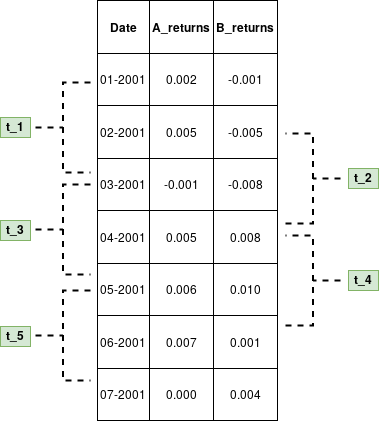
\includegraphics[width=.50\textwidth]{Bilder/rolling_window.png}
    \caption{Illustration of the rolling-window approach for a time-series containing seven time-steps filled with mock-data. Five subsets of length 3 divide the time-series.}
    \label{fig:rolling_window}
  \end{center}
\end{figure}
This approach is schematically described in figure \ref{fig:rolling_window}.\\

Finally, for each subset $t_i$, the weights are computed by solving the system of linear equations as in \ref{eq:9}. Out-of-sample excess returns are then calculated using the actual excess returns of the $i+1$'th time-step in an attempt to validate if a prediction in the past had been successful.\\

Lastly, the out-of-sample returns' arithmetic mean $\hat{\mu}$is devided by its standard deviation $\hat{\sigma}$ to derive the out-of-sample Sharpe ratio like so:
\begin{equation}\label{eq:out-of-sample-sharpe}
\hat{SR} = \frac{\hat{\mu}}{\hat{\sigma}}
\end{equation}

\newpage

\section{Implementation}
In this section we want to display and discuss the implementation of the approach described in the previous chapter in the R programming language. We will compute several performance measures of the Minimal Variance Portfolio we're about to derive from the data.

\subsection{Datasets and data preparation}
The first dataset upon which this analysis is based is called "Ten sector portfolios of the S\&P 500 and the US equity market portfolio". It has been created by Roberto Wessels and was obtained from Mendeley Data\footnote{Data can be downloaded \href{https://data.mendeley.com/datasets/ndxfrshm74/3}{here}. It is also attached to this report.}. Note that for this dataset, it is necessary to substract the Treasury Bill-rates from each entry to obtain adjusted returns stripped of the risk-free rate. We call this dataset \textbf{TSP}.\\

The other dataset concerned is provided by Kenneth French and downloaded from his website\footnote{The dataset from Kenneth Frenchs' website can be downloaded \href{http://mba.tuck.dartmouth.edu/pages/faculty/ken.french/ftp/F-F_Research_Data_Factors_CSV.zip}{here} and is also attached to this report.}. The dataset is called "SMB and HML portfolios and the US equity market portfolio" and contains the factors "Small Minus Big" (SMB) and "High Minus Low" (HMB) from the Fama-French three-factor model \footnote{For an introduction to the Fama-French three-factor model, see \href{https://en.wikipedia.org/wiki/Fama\%E2\%80\%93French_three-factor_model}{Wikipedia}.} as well as the whole S\&P500 portfolio. We call this dataset short \textbf{SHS} This dataset is already cleared from the risk-free rate, thus a Treasure Bill-rate adjustment is not necessary. \\

In listing \ref{code:0}, it is showcased how data is imported and loaded into a dataframe. In line 1, the .csv-file containing the data is loaded via the \lstinline|read.csv| function, where a separator as well as the header-parameter are specified. 

\begin{lstlisting}[caption={Loading the data and subtracting the risk-free rate from the columns of returns yields a dataframe containing the matrix of excess-returns.}, label=code:0, frame=single]
return_matrix = read.csv('../ten-roberto-wessels.csv', header=TRUE, sep=',')
sub_return_matrix = subset(return_matrix, select = -c(13))
sub_return_matrix = apply(sub_return_matrix[,-1], 2, '-', return_matrix[,13])
return_matrix = cbind(return_matrix$Date, sub_return_matrix)
colnames(return_matrix)[1] = 'Date'
\end{lstlisting}
In case of dataset TSP, it is necessary to subtract the risk-free rate from the returns. To do this, a subset of the return\_matrix is created in line 2, excluding the monthly risk-free rate which is stored in column 13 of the return\_matrix. In line 3, the risk-free rate is sutracted from every column the return\_matrix' subset, except for the column containing the date. Line 4 shows the reconstruction of the return\_matrix, now containing risk-free returns. After the dates' column-name has been reset in line 5, the return\_matrix now contains only risk-free returns. 

\subsection{Computing the in-sample Sharpe ratio}
A very basic way of measuring portfolio performance is provided by the in-sample Sharpe ratio. By setting $\tau = \lbrace 1, 2, \dots, T \rbrace$, the entire time-series is considered when computing the covariance matrix of the matrix of excess-returns $\Sigma_t$, effectively removing the weight-vectors' time-dependency. \\

Following the procedure leading to the system of linear equations in equation\ref{eq:9}, we first compute a covariance matrix of the entire risk-free return-matrix. Line 1 of listing \ref{code:is-sharpe-ratio} does just this, excluding the column containing the time-series dates. A vector of dimension equal to the amount of assets listed in the return\_matrix is constructed, where every component of the vector equals one.\\

\begin{lstlisting}[caption={This example shows how the in-sample Sharpe ratio for a matrix of expected returns, computed in the R programming language.}, label=code:is-sharpe-ratio, frame=single]
cov_return_matrix = cov(return_matrix[,-1])
b = vector(length=nA) + 1
weights = solve(cov_benchmark_matrix, b)
weights = weights/abs(sum(weights))
mean_returns = data.matrix(apply(benchmark_matrix[,-1], 2, mean))
weights = data.matrix(weights)
Sharpe_ratio_IS = t(mean_returns) %*% weights / sqrt(t(weights)%*%cov_benchmark_matrix%*%weights)
print(Sharpe_ratio_IS)
\end{lstlisting}

Line 3 of listing \ref{code:is-sharpe-ratio} uses the \lstinline|solve()| function to solve the linear equation by inverting the covariance matrix. The resulting \lstinline|weights|-vector is normalized in line 4. A vector containing the mean-values of \lstinline|return_matrix| is created in line 5 and the \lstinline|weights|-vector is converted to a data.matrix in line 6. This is done to facilitate the vector- and matrix-multiplication performed in line 7 to calculate the in-sample Sharpe ratio according to equation \ref{eq:in-sample-sharpe}, which is printed in line 7.\\

\subsection{Computing the out-sample Sharpe ratio} \label{subsec:minVar-out-sample-sharpe}
For computing the out-sample Sharpe ratio as described in section \ref{subsec:out-sample-sharpe-ratio}, the approach for deriving the in-sample Sharpe ratio needs to be altered to incorporate time-dependency. \\

Considering listing \ref{code:os-sharpe-ratio}, in lines 1 and 2, the number of assets as well as the length of the time-series are assigned respectively. \lstinline|M| contains the length of the rolling-sample, the iterator-variable \lstinline|t| is initialized in line 4 and adjusted to \lstinline|M|.\\

\begin{lstlisting}[caption={Computing the out-sample Sharpe ratio from the matrix of expected returns in R.}, label=code:os-sharpe-ratio, frame=single]
nA = dim(return_matrix[,-1])[2] # number of assets
T = dim(return_matrix)[1] # no of months
M = 120 # size of rolling-sample
t = M + 1 # adjust t_0 to size of rolling-sample
while (t <= T - 1) {
  tStart = t - M 
  tEnd = t 
  return_matrix_future = return_matrix[c(tEnd+1),] 
  cov_return_matrix_t = cov(data.matrix(return_matrix[c(tStart:tEnd),-1])) 
  b_t = vector(length=nA) + 1 
  x_t = solve(cov_return_matrix_t, b_t) 
  x_t = x_t/sum(x_t)
  
  if(t == M+1) { 
    history_of_weights = data.frame(t(x_t))
    mu = data.frame(return_matrix[,1][t], x_t %*% return_matrix_future[-1])
  }
  else {
    history_of_weights = rbind(history_of_weights, x_t)
    mu = rbind(mu, data.frame(return_matrix[,1][t], x_t %*% return_matrix_future[-1]))
  }
  t = t+1
}
\end{lstlisting}

In line 5, the sample gets rolling: By setting a \lstinline|while|-loop, we iterate over the whole time-series. The last date included in the rolling-sample is T-1, since it is the last value for which the expected returns of the next month are known. From line 6 to 12, the weights for time t $x_t$ are computed. They are stored in dataframe mu in line 15 and 19 respectively. Meanwhile, the weights are saved in a dataframe in line 15 and 19.

\newpage

\section{Discussion}
To validate the implementations of the minimum-variance portfolio, in this section metrices derived from the data will be compared with results from DeMiguel et al.\cite{DEM09}. Additionally, results will be graphically displayed and compared.\\

\subsection{Graphical Analysis}
As a first graphical display of results, a portfolio appreciation graph is constructed by cumulatively summing the returns and scaling them by a factor 100. Is is similar to having invested 100\$ in a specific portfolio at the beginning of the time-series considered. In figure \ref{fig:appreciation_graph}, the portfolio appreciation graph of the minimum variance portfolio, which has been created in previous chapter \ref{subsec:minVar-out-sample-sharpe}, as well as the portfolio appreciation graph of the naive investing strategy are displayed. When applicating a naive investing strategy as in \cite{DEM09}, the weight-vector $w_{naive}$ is of dimension $N$ and every component of $w_{naive}$ is of value $1/N$, where $N$ is the number of assets considered.

\begin{figure}[h]
  \begin{center}
    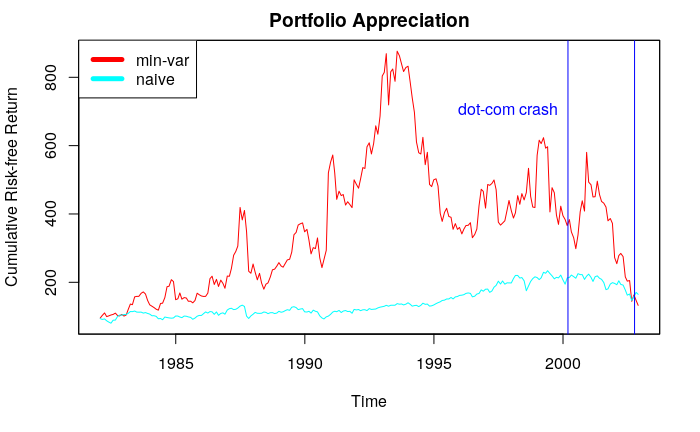
\includegraphics[width=\textwidth]{Bilder/portfolio-appreciation.png}
    \caption{The graph shows cumulative returns of two portfolio strategies: a naive portfolio (naive) and a minimum variance portfolio (min-var) as implemented in previous sections. The dataset on which the analysis was performed is SHS by Roberto Wessels.}
    \label{fig:appreciation_graph}
  \end{center}
\end{figure}

As can be seen in figure \ref{fig:appreciation_graph}, the minimum variance portfolio yields for a vast majority of time-steps considerably higher returns than the naive approach. This is especially evident in the period from 1990 to 1995. \\

\begin{table}[htbp]
  \begin{center}
    \begin{tabular}{|l|l|l|}
    \hline
     & Minimum variance portfolio & Naive portfolio \\ \hline
    mean cumulative return (per cent) & 362.75 & 142.72 \\ \hline
    maximum cumulative return (per cent) & 876.41 & 233.97 \\ \hline
    minimum cumulative return (per cent) & 95.52 & 80.36 \\ \hline
    \end{tabular}
  \end{center}
  \caption{Key data of the naive portfolio strategy as well as the minimum variance portfolio. The size of the rolling window to compute the minimum variance portfolio is set to 12 months.}
  \label{tab:portfolio-appreciation}
\end{table}

However, during the dot-com crash, which lasted from March 11, 2000 to October 9, 2002\footnote{Dates taken from the \href{https://en.wikipedia.org/wiki/Dot-com_bubble}{wikipedia page of the dot-com bubble}.}, both portfolio-stategies lead to diminishing cumulative returns. Especially the minimum variance portfolio performs poorly during this period.\\

Table \ref{tab:portfolio-appreciation} summarizes the results. It becomes evident that the minimum variance portfolio performed on this dataset in a superior fashion compared to the naive portfolio. The absolute minimum cumulative return is about 15\% lower for the minimum variance portfolio compared to the naive portfolio. The maximum cumulative return accomplished is roughly 3 times higher and the mean cumulative return approximately twice as big when emplozing a minimum variance portfolio compared to a portfolio following the naive approach.\\

\begin{figure}[h]
  \begin{center}
    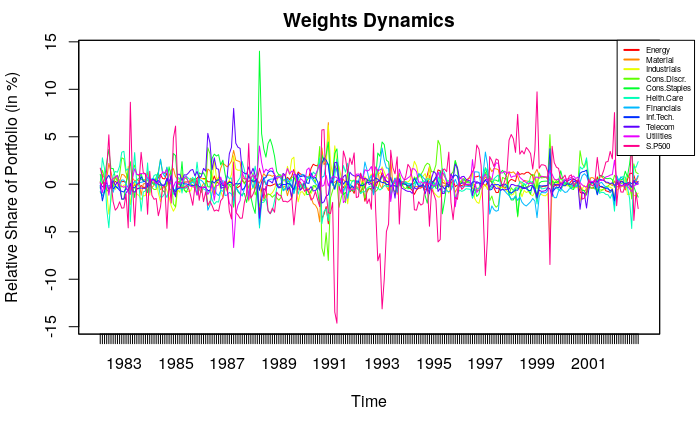
\includegraphics[width=\textwidth]{Bilder/dynamics-of-weights.png}
    \caption{This figure depicts the dynamics of weights of a minimum variance portfolio as implemented in previous sections. The size of the rolling-window is set to 12 months. The dataset considered is SHS by Roberto Wessels.}
    \label{fig:dynamics_of_weights}
  \end{center}
\end{figure}

Figure \ref{fig:dynamics_of_weights} shows the weights' dependency on time. Since the weights are normalized (compare with listing \ref{code:os-sharpe-ratio}, line 12), any single weight larger than 1 (or -1) implies that additional capital shall be lended to either further buy stock (if the weight is bigger than 0) or to sell short the correpsonding stock. As can be expected for a minimum variance portfolio, the weights fluctuate heavily over time.\\

\subsection{Comparing numerical results}
This work was motivated by the paper \glqq Optimal versus naive diversification: how inefficient is the 1/$N$ portfolio strategy?\grqq~by DeMiguel et al. \cite{DEM09}. The two datasets used for the analysis in this report were also used by DeMiguel et al., thus a comparison of results seems logical.\\

\begin{table}[h]
  \begin{center}
    \begin{tabular}{|l|l|l|}
    \hline
    Strategy & TSP &  SHS\\ \hline
    min\textsubscript{DM}& 0.0820 & 0.2493\\ \hline
    min\textsubscript{OS} & 0.0386 & 15.5675 \\ \hline
    min\textsubscript{IS} & 0.0588 & 0.2461 \\ \hline
    \end{tabular}
  \end{center}
\caption{Comparison of the Sharpe ratios of the minimum variance portfolio strategy. Values of strategies with subscript \glqq DM\grqq~are taken from DeMiguel et al. Strategies with subscript \glqq OS\grqq~name the out-sample Sharpe ratios computed by the author of this report, subscript \glqq IS\grqq~denote in-sample Sharpe ratios.} 
\label{tab:comparison-sharpe-ratios}
\end{table}

Table \ref{tab:comparison-sharpe-ratios} lists all Sharpe ratios taken from DeMiguel et al. \cite{DEM09} and also values computed by the author of this report. While in the original paper, the authors chose to only publish the out-sample Sharpe ratio, in-sample Sharpe ratios were also computed and listed in table \ref{tab:comparison-sharpe-ratios} within brackets. \\

It can be seen that the results differ more or less strongly from the results obtrained by DeMiguel et al. While the out-sample Sharpe ratio for the SHS-dataset is off by two orders of magnitude, the in-sample Sharpe ratio has an relative deviation from the DeMiguel et al.-result by 1.2\%.\\

Meanwhile, the deviation from the original paper's result for the TSP-dataset is 52.9\% for the out-sample Sharpe ratio and 28.3\% for the in-sample Sharpe ratio. \\

The error for the TSP-dataset might be explicable by the fact that the data might not be the same as DeMiguel et al. used in their study. It was obtained from an unofficial source\footnote{Data can be downloaded \href{https://data.mendeley.com/datasets/ndxfrshm74/3}{here}} and could be faulty. \\

Meanwhile, dataset SHS was directly obtained from the same source used by DeMiguel et al. The difference by two orders of magnitude between in-sample and out-sample Sharpe ratio is surprising. This hints at a systematic error in the computation of out-sample Sharpe ratios.

\newpage

\section{Conclusion}
In this report, the minimum variance portfolio strategy has been elaborated. In a theoretical chapter, basic portfolio-theoretical concepts were discussed. Constraints for the minimum variance portfolio strategy were introduced and explained. In a next step, an optimization problem was derived from the portfolio constraints. The problem was transformed to a linear system of equations, which can be solved by inverting a matrix. In-sample and out-sample Sharpe ratio were introduced as important measures of performance. \\

Datasets, their sources, meanings and relevance were introduced. The subtraction of treasure-bill rates from the returns was discussed and demonstrated. \\

In the following section, implementations of theoretical core-concepts in the R programming language were discussed. The programmatical difference between in-sample Sharpe ratio and out-sample Sharpe ratio was thusly accentuated.\\

Graphical results were shown and discussed. The superiority of the minimum variance portfolio in comparison to the naive portfolio was stressed and fortified by key data extracted from the computed returns. The weights' time sensitivity was displayed in a weights dynamics graph.\\

Finally, numerical results were compared to results obtained by DeMiguel et al \cite{DEM09}.

\section{Appendix}
What follows is the full souce-code listing.
\begin{lstlisting}[label=code:full-source-code, frame=single]
return_matrix_eleven = read.csv('../ten-roberto-wessels.csv', header=TRUE, sep=',')
return_matrix_three = read.csv('../two-plus-one.csv', header=TRUE, sep = ',')
colnames(return_matrix_three)[1] = 'Date'

# data-cleaning: subtracting the tbill-rate from returns
sub_return_matrix = subset(return_matrix_eleven, select = -c(13))
sub_return_matrix = apply(sub_return_matrix[,-1], 2, '-', return_matrix_eleven[,13])
return_matrix_eleven = cbind(return_matrix_eleven$Date, sub_return_matrix)
colnames(return_matrix_eleven)[1] = 'Date'

# function calcMinVarWeights expects a matrix of returns, where the first column
# contains an index (e.g. date) and all other columns contain returns.
# the function returns a normalized weights vector
calcMinVarWeights = function(return_matrix) {
  return_matrix = data.matrix(return_matrix) # convert for applying linear algebra
  
  # solve system of linear equations
  nA = dim(return_matrix[,-1])[2] # number of assets
  b = vector(length=nA) + 1 # constraint-vector
  cov_matrix = cov(return_matrix[,-1]) # dates are deleted
  weights = solve(cov_matrix, b)
  weights = data.matrix(weights/sum(weights)) # normalize the vector
  
  return (weights)
}

# the function inSamplesharpe expects a data frame, where the first column is 
# contains an index and returns the in-sample Sharpe ratio of said data frame.
inSampleSharpe = function(return_matrix) {
  
  # calculate weights
  weights = calcMinVarWeights(return_matrix)
  
  # calculate mean of each asset
  mean_returns = data.matrix(apply(return_matrix[,-1], 2, mean)) 
  
  # calculate sharpe-ratio according to formula
  cov_matrix = cov(return_matrix[,-1])
  sharpe_ratio_in_sample = 
  t(mean_returns) %*% weights/ sqrt(t(weights)%*%cov_matrix%*%weights)
  
  return (sharpe_ratio_in_sample)
}

### results for both datasets ###
sharpe_ratio_IS_three = inSampleSharpe(return_matrix_three)
sharpe_ratio_IS_eleven = inSampleSharpe(return_matrix)
sharpe_ratio_IS_three
sharpe_ratio_IS_eleven

# the function outSampleSharpe expects a return_matrix where the first column
# contains an index (e.g. a Date) and all other columns contain returns.
# parameter M (int) indicates the size of the rolling-sample
# parameter historyOfWeights (boolean) indicates if instead of a data frame
# with columns date, minvar-returns, cumulative minvar-returns 
# and cumulative naive-returns a data frame containing the weights should be 
# returned
outSampleSharpe = function(return_matrix, M, historyOfWeights) {
  return_matrix = data.matrix(return_matrix)
  nA = dim(return_matrix[,-1])[2] # number of assets
  T = dim(return_matrix)[1] # no of months
  t = M + 1 # adjust t_0 to size of rolling-sample
  b = vector(length=nA) + 1 # set up restraints_vector
  while (t <= T - 1) {
    tStart = t - M # lower barrier for the time-interval
    tEnd = t # upper barrier for the time-interval
    return_matrix_future = return_matrix[c(tEnd+1),] # return matrix t+1 in the future
    
    cov_return_matrix_t = cov(data.matrix(return_matrix[c(tStart:tEnd),-1])) # calculate cov-matrix for time t
    w_t = solve(cov_return_matrix_t, b) # solve system of equations
    w_t = w_t/sum(w_t) # normalize weights
  
    ## calculate returns
    ret_t = w_t %*% return_matrix_future[-1] #min-var returns
    naive_ret_t = (vector(length=nA) + 1/nA) %*% return_matrix_future[-1] #naive returns
  
    if(t == M+1) { # in the first iteration, create df
      if(historyOfWeights) {
            mu = data.frame(t(w_t))
      } else {
      mu = data.frame(return_matrix[,1][t], 
                      ret_t, 100 * (1 + ret_t), 
                      100 * (1 + naive_ret_t))
      colnames(mu) = c('Date', 
                       'returns', 
                       'cumulative returns', 
                       'naive cumulative returns')
        }
      } else {
        if(historyOfWeights) {
              # save weights
              mu = rbind(mu, w_t)
        } else {
          # calculate cumulative return
          cumul_ret = mu[tStart-1,3] * (1 + ret_t)
          naive_cumul_ret = mu[tStart-1,4] * (1 + naive_ret_t)
          # save returns
          new = data.frame(return_matrix[,1][t], 
                           ret_t, 
                           cumul_ret, 
                           naive_cumul_ret)
          colnames(new) = c('Date', 
                            'returns', 
                            'cumulative returns', 
                            'naive cumulative returns')
          mu = rbind(mu, new)
        }
    }
    t = t+1
    }
  return (mu)
}
mu_three = outSampleSharpe(return_matrix_three, 120, FALSE)
mu_eleven = outSampleSharpe(return_matrix_eleven, 120, FALSE)
mean(mu_three$returns) / var(mu_three$returns)
mean(mu_eleven$returns) / var(mu_eleven$returns)

library('zoo')
library('xts')
history_of_returns = data.frame(as.Date(as.character(mu$Date), format="%Y%m%d"), mu[,c(2:4)])
colnames(history_of_returns) = c('Date', 'Out-of-sample returns', 'cumulative returns', 'naive cumulative returns')
View(portfolio_appreciation)
portfolio_appreciation = as.xts(history_of_returns[,c(-1,-2)], order.by=history_of_returns$Date)
zoo.appreciation = as.zoo(portfolio_appreciation)
cumretRainbow = rainbow(ncol(zoo.appreciation))
{plot.zoo(x = zoo.appreciation, main = 'Portfolio Appreciation', xlab='Time', ylab='Cumulative Risk-free Return (in %)', col = cumretRainbow, screens = 1)
legend(x = "topleft", legend = c("min-var", "naive"), lwd=5, col = cumretRainbow)
abline(v = c(as.Date('2000-03-11'), as.Date('2002-10-09')), col= 'blue')
text(x = as.Date('2000-03-01'), y=700, pos = 2, labels = 'dot-com crash', col='blue')
}

min(portfolio_appreciation$`cumulative returns`)
mean(portfolio_appreciation$`cumulative returns`)
max(portfolio_appreciation$`cumulative returns`)
mean(portfolio_appreciation$`naive cumulative returns`)
max(portfolio_appreciation$`naive cumulative returns`)
min(portfolio_appreciation$`naive cumulative returns`)

history_of_weights = outSampleSharpe(return_matrix_eleven, 12, TRUE)
weightsHistoryDf = data.frame(return_matrix[14:dim(return_matrix)[1],1], history_of_weights)
colnames(weightsHistoryDf)[1] = "Date"

weightsHistoryDf$Date = as.yearmon(as.character(weightsHistoryDf$Date), format="%Y%m")
weightsHistoryXts = as.xts(weightsHistoryDf[,-1], order.by=weightsHistoryDf$Date)
zoo.weightsHistory = as.zoo(weightsHistoryXts)
View(zoo.weightsHistory)
weightsRainbow = rainbow(ncol(zoo.weightsHistory))
{
par(xpd=TRUE)
plot(zoo.weightsHistory, main='Weights Dynamics', xlab='Time', ylab='Relative Share of Portfolio (in %)', screens=1, col=weightsRainbow, xpd=TRUE)
legend(x = "topright", legend = colnames(weightsHistoryDf)[c(2:12)], lwd=2, col = weightsRainbow, inset=c(-0.06,0), xpd=TRUE, pt.cex = 1, cex = 0.5)}
\end{lstlisting}